\section{Exponential Distribution}
\label{sec:Exponential-Distribution}

The arrival and service processes can follow whichever probabilistic distribution. Most often, inter-arrival and service times follow the exponential distribution, because of its wide applicability and mathematical tractability.
The Exponential distribution is the continuous counterpart of the Geometric distribution. The Geometric distribution models the number of attempts until the first success, whereas the Exponential distribution models the time until the first success.

\begin{definition}[Exponential Distribution]
\label{def:Exponential-Distribution}	
	A random variable $X$ is Exponentially distributed with rate\footnote{if $X \sim Exp(\lambda)$, $\lambda$ is called \textit{rate} because $\expected{X}=\frac{1}{\lambda}$.} $\lambda$ ($X \sim Exp(\lambda)$) if $X$ has the following probability density function:
	
	\begin{equation}
	\label{eqn:Exponential-PDF}
	f(x) = \left\{\begin{matrix}
		\lambda e^{-\lambda x} & x \geq 0\\ 
		0 & x \leq 0
	\end{matrix}\right.
	\end{equation}
\end{definition}

The p.d.f of $X \sim Exp(\lambda)$ is shown in \Cref{fig:Exponential-PDF}.

\begin{figure}[tp]
\label{fig:Exponential-PDF}	
	\centering
	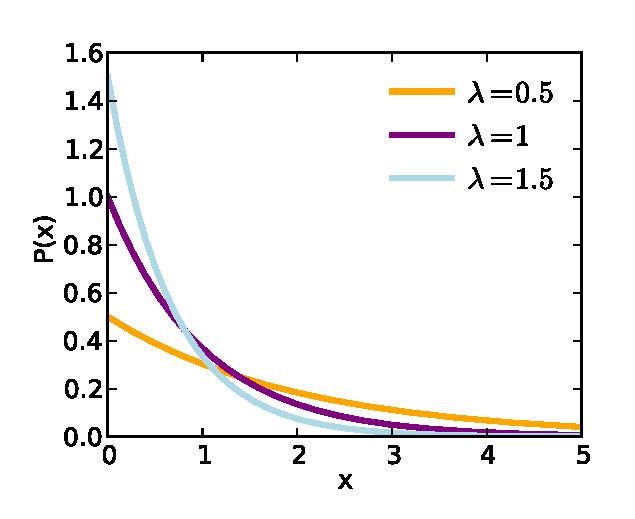
\includegraphics{fig/exponential-pdf}
	\caption{Exponential p.d.f.}
\end{figure}

From the \Cref{def:Exponential-Distribution} follows that the cumulative distribution function of $X \sim Exp(\lambda)$ is

\begin{equation}
\label{eqn:Exponential-CDF}
\begin{aligned}
	F(x) = \int_{- \infty}^{x} \partial y = 
	\left\{\begin{matrix}
	1 - e^{-\lambda x} & x \geq 0\\ 
	0 & x \leq 0
	\end{matrix}\right.
\end{aligned}
\end{equation}

The Exponential distribution has moments

\begin{equation}
\label{eqn:Exponential-Mean}
\expected{X} = \int_{- \infty}^{\infty} xf(x) \partial x = \frac{1}{\lambda}
\end{equation}

\begin{equation}
\label{eqn:Exponential-Moment-2}
\expected{X^{2}} = \int_{- \infty}^{\infty} x^{2}f(x) \partial x = \frac{2}{\lambda^{2}}
\end{equation}

and variance

\begin{equation}
\label{eqn:Exponential-Variance}
	\variance{X} = \expected{X^{2}} - \expected{X}^{2} = \frac{1}{\lambda^{2}}
\end{equation}

The Exponential distribution is so convenient because it is memoryless. In particular, the Exponential distribution is the only continuous memoryless distribution.

\begin{theorem}[Exponential Memoryless]
\label{thm:Exponential-Memoryless}

	A random variable $X \sim Exp(\lambda)$ is memoryless.
	
	\begin{proof}
		\begin{equation*}
		\probability{X > s+t | X > s}=\frac{X > s+t}{X > s}=\frac{e^{- \lambda (s+t)}}{e^{- \lambda s}}=e^{- \lambda t}=\probability{X > t}
		\end{equation*}
	\end{proof}
\end{theorem}

The Exponential distribution is memoryless and with constant failure rate. It exposes also the following useful properties.

\begin{theorem}[Precedency of Exponentials]
\label{thm:Exponential-Precedency}
	Given independent $X_{1} \sim Exp(\lambda_{1})$ and $X_{2} \sim Exp(\lambda_{2})$, we have that
	
	\begin{equation}
	\label{eqn:Exponential-Precedency}
	\probability{X_{1} < X_{2}} = \frac{\lambda_{1}}{\lambda_{1} + \lambda_{2}}
	\end{equation}
\end{theorem}

\begin{theorem}[Minimum Exponentials]
\label{thm:Exponential-Minimum}
	Given independent $X_{1} \sim Exp(\lambda_{1})$ and $X_{2} \sim Exp(\lambda_{2})$, we have that
	
	\begin{equation}
	\label{eqn:Exponential-Minimum}
	\min(X_{1},X_{2}) \sim Exp(\lambda_{1} + \lambda_{2})
	\end{equation}
\end{theorem}